\documentclass{standalone}
\usepackage{tikz}
\usetikzlibrary{patterns, positioning}
\usepackage[sfdefault]{ClearSans} %% option 'sfdefault' activates Clear Sans as the default text font
\usepackage[T1]{fontenc}

\begin{document}
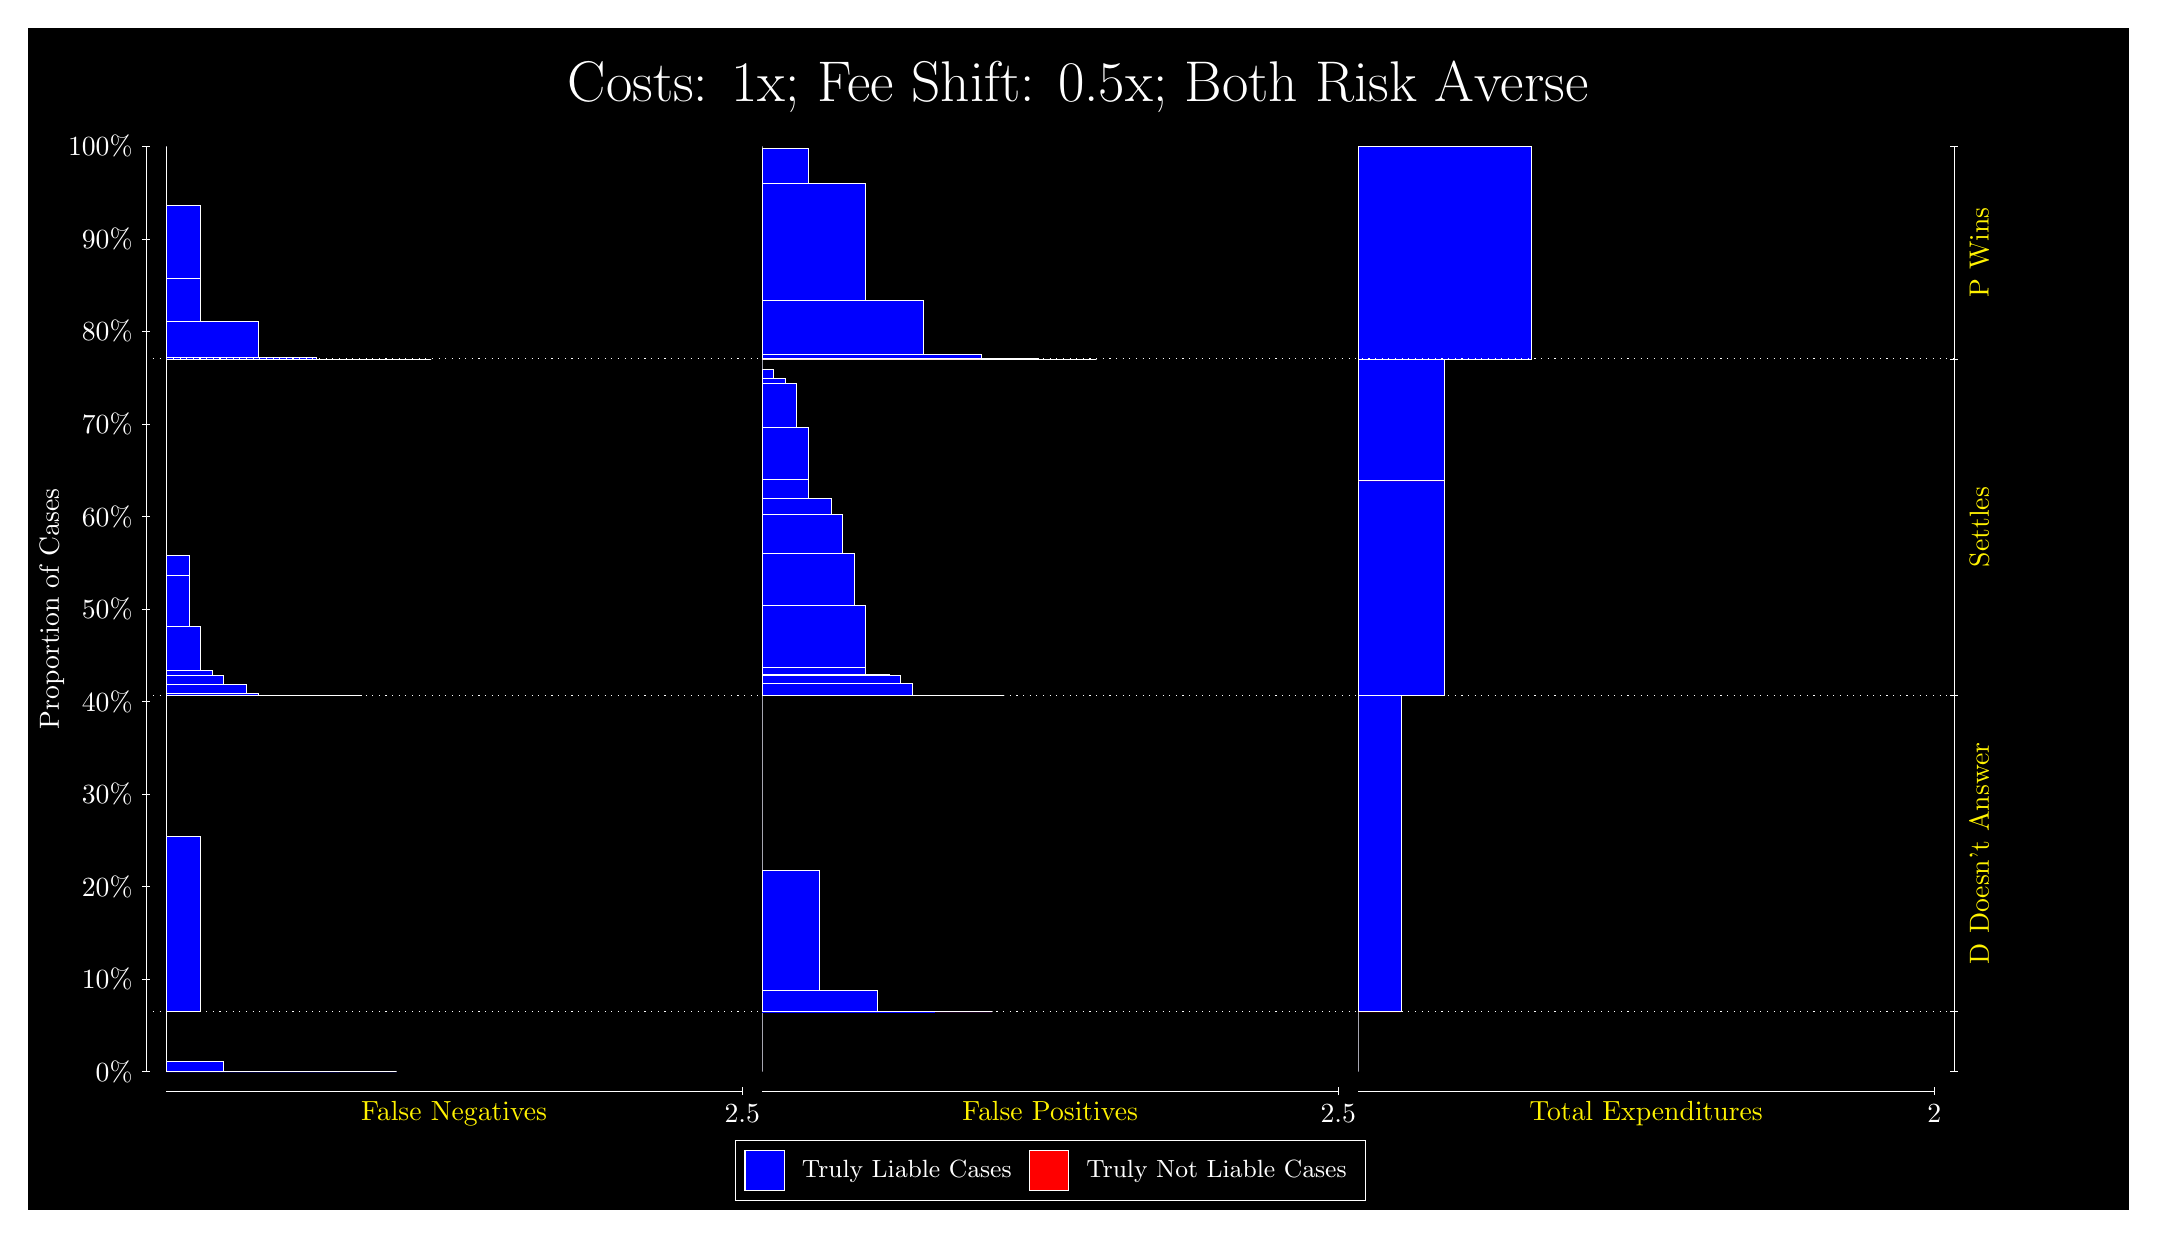
\begin{tikzpicture}
\draw[fill=black] (0,0) rectangle (26.667,15);
\draw[text=white] (0,13.5) rectangle (26.667,15) node[midway] {\huge Costs: 1x; Fee Shift: 0.5x; Both Risk Averse};
\draw[white, very thin] (1.5,1.75) -- (1.5,13.5);
\node[rotate=90, text=white, anchor=center] at (0.3, 7.625) {Proportion of Cases};
\draw[white, very thin] (1.45,1.75) -- (1.55,1.75);
\node[text=white, anchor=east] at (1.45, 1.75) {0\%};
\draw[white, very thin] (1.45,2.925) -- (1.55,2.925);
\node[text=white, anchor=east] at (1.45, 2.925) {10\%};
\draw[white, very thin] (1.45,4.1) -- (1.55,4.1);
\node[text=white, anchor=east] at (1.45, 4.1) {20\%};
\draw[white, very thin] (1.45,5.275) -- (1.55,5.275);
\node[text=white, anchor=east] at (1.45, 5.275) {30\%};
\draw[white, very thin] (1.45,6.45) -- (1.55,6.45);
\node[text=white, anchor=east] at (1.45, 6.45) {40\%};
\draw[white, very thin] (1.45,7.625) -- (1.55,7.625);
\node[text=white, anchor=east] at (1.45, 7.625) {50\%};
\draw[white, very thin] (1.45,8.8) -- (1.55,8.8);
\node[text=white, anchor=east] at (1.45, 8.8) {60\%};
\draw[white, very thin] (1.45,9.975) -- (1.55,9.975);
\node[text=white, anchor=east] at (1.45, 9.975) {70\%};
\draw[white, very thin] (1.45,11.15) -- (1.55,11.15);
\node[text=white, anchor=east] at (1.45, 11.15) {80\%};
\draw[white, very thin] (1.45,12.325) -- (1.55,12.325);
\node[text=white, anchor=east] at (1.45, 12.325) {90\%};
\draw[white, very thin] (1.45,13.5) -- (1.55,13.5);
\node[text=white, anchor=east] at (1.45, 13.5) {100\%};

\draw[white, very thin] (24.457,1.75) -- (24.457,13.5);
\draw[white, very thin] (24.407,1.75) -- (24.507,1.75);
\node[anchor=west] at (24.407, 1.75) {};
\draw[white, very thin] (24.407,2.5101) -- (24.507,2.5101);
\node[anchor=west] at (24.407, 2.5101) {};
\draw[white, very thin] (24.407,6.5295) -- (24.507,6.5295);
\node[anchor=west] at (24.407, 6.5295) {};
\draw[white, very thin] (24.407,10.801) -- (24.507,10.801);
\node[anchor=west] at (24.407, 10.801) {};
\draw[white, very thin] (24.407,13.5) -- (24.507,13.5);
\node[anchor=west] at (24.407, 13.5) {};

\draw[white, very thin, fill=blue] (1.75,1.75) rectangle (4.6775,1.75);
\draw[white, very thin, fill=blue] (1.75,1.75) rectangle (3.9457,1.75);
\draw[white, very thin, fill=blue] (1.75,1.75) rectangle (3.2138,1.7511);
\draw[white, very thin, fill=blue] (1.75,1.7511) rectangle (2.4819,1.8745);
\draw[white, very thin, fill=red] (1.75,1.8745) rectangle (1.75,1.8745);
\draw[white, very thin, fill=blue] (1.75,1.8745) rectangle (1.75,2.5101);
\draw[white, very thin, fill=blue] (1.75,2.5101) rectangle (2.1891,4.7328);
\draw[white, very thin, fill=red] (1.75,4.7328) rectangle (1.75,4.7328);
\draw[white, very thin, fill=blue] (1.75,4.7328) rectangle (1.75,6.5295);
\draw[white, very thin, fill=blue] (1.75,6.5295) rectangle (4.2384,6.5295);
\draw[white, very thin, fill=blue] (1.75,6.5295) rectangle (3.6529,6.5295);
\draw[white, very thin, fill=blue] (1.75,6.5295) rectangle (3.5065,6.5297);
\draw[white, very thin, fill=blue] (1.75,6.5297) rectangle (3.0674,6.5298);
\draw[white, very thin, fill=blue] (1.75,6.5298) rectangle (2.921,6.5496);
\draw[white, very thin, fill=blue] (1.75,6.5496) rectangle (2.7746,6.6674);
\draw[white, very thin, fill=blue] (1.75,6.6674) rectangle (2.4819,6.7776);
\draw[white, very thin, fill=blue] (1.75,6.7776) rectangle (2.3355,6.8448);
\draw[white, very thin, fill=blue] (1.75,6.8448) rectangle (2.1891,7.3985);
\draw[white, very thin, fill=blue] (1.75,7.3985) rectangle (2.0428,8.0564);
\draw[white, very thin, fill=blue] (1.75,8.0564) rectangle (2.0428,8.3025);
\draw[white, very thin, fill=red] (1.75,8.3025) rectangle (1.75,8.3025);
\draw[white, very thin, fill=blue] (1.75,8.3025) rectangle (1.75,10.801);
\draw[white, very thin, fill=blue] (1.75,10.801) rectangle (5.1167,10.801);
\draw[white, very thin, fill=blue] (1.75,10.801) rectangle (4.3848,10.801);
\draw[white, very thin, fill=blue] (1.75,10.801) rectangle (3.6529,10.826);
\draw[white, very thin, fill=blue] (1.75,10.826) rectangle (2.921,11.272);
\draw[white, very thin, fill=blue] (1.75,11.272) rectangle (2.1891,11.826);
\draw[white, very thin, fill=blue] (1.75,11.826) rectangle (2.1891,12.753);
\draw[white, very thin, fill=red] (1.75,12.753) rectangle (1.75,12.753);
\draw[white, very thin, fill=blue] (1.75,12.753) rectangle (1.75,13.5);
\draw[white, very thin, fill=red] (9.3189,1.75) rectangle (9.3189,1.75);
\draw[white, very thin, fill=blue] (9.3189,1.75) rectangle (9.3189,2.5101);
\draw[white, very thin, fill=red] (9.3189,2.5101) rectangle (12.246,2.5101);
\draw[white, very thin, fill=blue] (9.3189,2.5101) rectangle (12.246,2.5101);
\draw[white, very thin, fill=blue] (9.3189,2.5101) rectangle (11.515,2.5123);
\draw[white, very thin, fill=blue] (9.3189,2.5123) rectangle (10.783,2.7813);
\draw[white, very thin, fill=blue] (9.3189,2.7813) rectangle (10.051,4.3068);
\draw[white, very thin, fill=blue] (9.3189,4.3068) rectangle (9.3189,6.5295);
\draw[white, very thin, fill=red] (9.3189,6.5295) rectangle (12.393,6.5295);
\draw[white, very thin, fill=blue] (9.3189,6.5295) rectangle (12.393,6.5295);
\draw[white, very thin, fill=red] (9.3189,6.5295) rectangle (12.1,6.5295);
\draw[white, very thin, fill=blue] (9.3189,6.5295) rectangle (12.1,6.5295);
\draw[white, very thin, fill=red] (9.3189,6.5295) rectangle (11.807,6.5295);
\draw[white, very thin, fill=blue] (9.3189,6.5295) rectangle (11.807,6.5297);
\draw[white, very thin, fill=blue] (9.3189,6.5297) rectangle (11.661,6.5297);
\draw[white, very thin, fill=blue] (9.3189,6.5297) rectangle (11.368,6.5305);
\draw[white, very thin, fill=red] (9.3189,6.5305) rectangle (11.222,6.5305);
\draw[white, very thin, fill=blue] (9.3189,6.5305) rectangle (11.222,6.6782);
\draw[white, very thin, fill=blue] (9.3189,6.6782) rectangle (11.075,6.7821);
\draw[white, very thin, fill=blue] (9.3189,6.7821) rectangle (10.929,6.7893);
\draw[white, very thin, fill=blue] (9.3189,6.7893) rectangle (10.636,6.8858);
\draw[white, very thin, fill=red] (9.3189,6.8858) rectangle (10.636,6.8858);
\draw[white, very thin, fill=blue] (9.3189,6.8858) rectangle (10.636,7.6679);
\draw[white, very thin, fill=blue] (9.3189,7.6679) rectangle (10.49,8.3259);
\draw[white, very thin, fill=blue] (9.3189,8.3259) rectangle (10.344,8.8226);
\draw[white, very thin, fill=blue] (9.3189,8.8226) rectangle (10.197,9.0278);
\draw[white, very thin, fill=blue] (9.3189,9.0278) rectangle (9.9044,9.2739);
\draw[white, very thin, fill=blue] (9.3189,9.2739) rectangle (9.9044,9.9319);
\draw[white, very thin, fill=blue] (9.3189,9.9319) rectangle (9.758,10.485);
\draw[white, very thin, fill=blue] (9.3189,10.485) rectangle (9.6116,10.553);
\draw[white, very thin, fill=blue] (9.3189,10.553) rectangle (9.4652,10.663);
\draw[white, very thin, fill=blue] (9.3189,10.663) rectangle (9.3189,10.801);
\draw[white, very thin, fill=red] (9.3189,10.801) rectangle (13.564,10.801);
\draw[white, very thin, fill=blue] (9.3189,10.801) rectangle (13.564,10.801);
\draw[white, very thin, fill=red] (9.3189,10.801) rectangle (12.832,10.801);
\draw[white, very thin, fill=blue] (9.3189,10.801) rectangle (12.832,10.802);
\draw[white, very thin, fill=red] (9.3189,10.802) rectangle (12.1,10.802);
\draw[white, very thin, fill=blue] (9.3189,10.802) rectangle (12.1,10.862);
\draw[white, very thin, fill=red] (9.3189,10.862) rectangle (11.368,10.862);
\draw[white, very thin, fill=blue] (9.3189,10.862) rectangle (11.368,11.548);
\draw[white, very thin, fill=red] (9.3189,11.548) rectangle (10.636,11.548);
\draw[white, very thin, fill=blue] (9.3189,11.548) rectangle (10.636,13.029);
\draw[white, very thin, fill=blue] (9.3189,13.029) rectangle (9.9044,13.475);
\draw[white, very thin, fill=blue] (9.3189,13.475) rectangle (9.3189,13.5);
\draw[white, very thin, fill=red] (16.888,1.75) rectangle (16.888,1.75);
\draw[white, very thin, fill=blue] (16.888,1.75) rectangle (16.888,2.5101);
\draw[white, very thin, fill=red] (16.888,2.5101) rectangle (17.437,2.5101);
\draw[white, very thin, fill=blue] (16.888,2.5101) rectangle (17.437,6.5295);
\draw[white, very thin, fill=red] (16.888,6.5295) rectangle (17.986,6.5295);
\draw[white, very thin, fill=blue] (16.888,6.5295) rectangle (17.986,9.256);
\draw[white, very thin, fill=red] (16.888,9.256) rectangle (17.986,9.256);
\draw[white, very thin, fill=blue] (16.888,9.256) rectangle (17.986,10.801);
\draw[white, very thin, fill=red] (16.888,10.801) rectangle (19.083,10.801);
\draw[white, very thin, fill=blue] (16.888,10.801) rectangle (19.083,13.5);
\draw[white, dotted] (1.5,2.5101) -- (24.457,2.5101);
\draw[white, dotted] (1.5,6.5295) -- (24.457,6.5295);
\draw[white, dotted] (1.5,10.801) -- (24.457,10.801);
\draw[white, very thin] (1.75,1.5) -- (9.0689,1.5);
\node[text=yellow, anchor=north] at (5.4094, 1.5) {False Negatives};
\draw[white, very thin] (9.0689,1.45) -- (9.0689,1.55);
\node[text=white, anchor=north] at (9.0689, 1.45) {2.5};

\draw[white, very thin] (9.3189,1.5) -- (16.638,1.5);
\node[text=yellow, anchor=north] at (12.978, 1.5) {False Positives};
\draw[white, very thin] (16.638,1.45) -- (16.638,1.55);
\node[text=white, anchor=north] at (16.638, 1.45) {2.5};

\draw[white, very thin] (16.888,1.5) -- (24.207,1.5);
\node[text=yellow, anchor=north] at (20.547, 1.5) {Total Expenditures};
\draw[white, very thin] (24.207,1.45) -- (24.207,1.55);
\node[text=white, anchor=north] at (24.207, 1.45) {2};


\node[text=yellow, centered, rotate=90] at (24.777, 4.5198) {D Doesn't Answer};
\node[text=yellow, centered, rotate=90] at (24.777, 8.6652) {Settles};
\node[text=yellow, centered, rotate=90] at (24.777, 12.15) {P Wins};

\draw (12.978300999999998,1.5) node[draw=none] (baseCoordinate) {};
\begin{scope}[align=center]
        \matrix[scale=0.5, draw=white, below=0.5cm of baseCoordinate, nodes={draw}, column sep=0.1cm]{
            \node[rectangle, draw, minimum width=0.5cm, minimum height=0.5cm, fill=blue] {}; &
            \node[draw=none, font=\small, text=white] (B) {Truly Liable Cases}; &
            \node[rectangle, draw, minimum width=0.5cm, minimum height=0.5cm, fill=red] {}; &
            \node[draw=none, font=\small, text=white] (B) {Truly Not Liable Cases}; \\
            };
\end{scope}

\end{tikzpicture}
\end{document}